%!TEX root = ../dissertation.tex

\chapter{Methods}

\newthought{The simulations described} in this thesis were carried out according to a new protocol for temperature-dependent calculation of vibrational spectra. This protocol consists of three phases: the sampling of molecular configurations, the simulation of molecular wavefunctions, the vibrational analysis of these wavefunctions, and the reconstruction of spectra from the analysis results. The three latter phases are well understood in the computational chemistry community\cite{RefWorks:33, RefWorks:34, RefWorks:37, RefWorks:38, RefWorks:39, RefWorks:40}, but the methods outlined here for the first phase are, to our knowledge, novel.

\section{Sampling Molecular Configurations}

Spectral simulation begins with a molecular geometry. This geometry is a set of three-dimensional coordinates that describe the type and spatial location of all the atoms in a molecule. Typically, computational chemistry assumes that the energy of the geometry is minimized\textemdash that is, that the atoms in the structure are arranged such that the potential energy stored in the molecule is as small as possible. While this simplifies calculations, it is not realistic. A molecule fixed at its minimum potential energy is at a virtual absolute zero, which is, in effect, the temperature at which most chemical calculations are carried out.

In reality, molecules are always at a nonzero temperature, and move through a large space of possible configurations. The temperature of the system to which a molecule belongs describes the size of this space; in general, the hotter a system is, the more possible configurations it can assume. Vibrations modulate a molecule through different geometries, and in turn those geometries constrain the ways in which a molecule can vibrate; it follows that molecules in a thermally excited state with access to high-energy geometries will vibrate differently and display different vibrational spectra than those which are frozen at absolute zero.

\begin{figure}
	\centering
	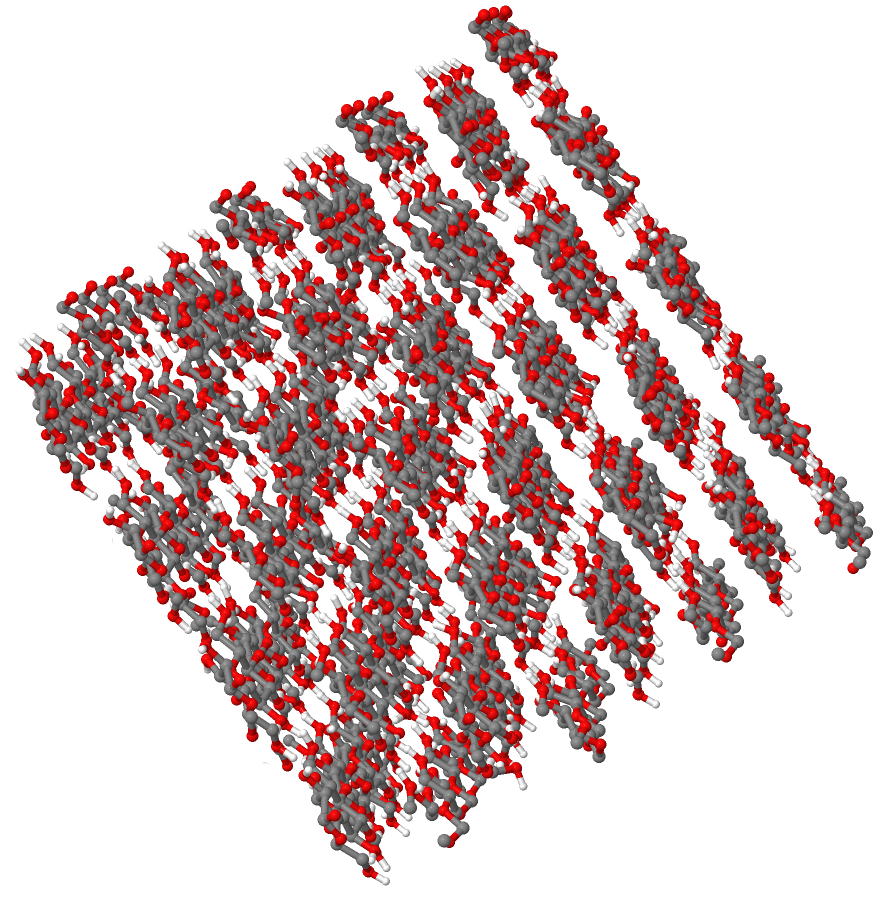
\includegraphics[width=0.7\linewidth]{md_cellulose}
	\caption{Snapshot of cellulose configuration from molecular dynamics simulation at 280K.}
	\label{fig:md_cellulose}
\end{figure}

To address this issue, we drew molecular geometries from the results of large-scale molecular dynamics (MD) simulations of cellulose. MD is a well-understood method for simulating large molecules and molecular systems using classical physics\cite{RefWorks:25}; it works by taking as input the locations and velocities of all the particles in the simulated system, then using a carefully selected potential function to calculate all the forces between the particles. These forces then determine how the particles move according to Newtonian mechanics, which in turn determine how the forces change, and so on. By iteratively evaluating the positions, velocities, and forces at successive discrete time steps separated by as little as a femtosecond, the behavior of molecules can be accurately simulated.

The particular MD approach employed here was designed and implemented by Vishal Agarwal expressly for the purpose of simulating cellulose \cite{RefWorks:23}. This simulation takes in temperature as a parameter, and models the behavior of more than 3,200 atoms in 32 strands of cellulose arranged in 8 parallel sheets for a period of 10 nanoseconds. This simulation is carried out by GROMACS, an open-source software package designed expressly for this type of work \cite{RefWorks:24}.

The molecules in this simulation bend, stretch, and warp according to their own thermal energy and the laws of Newtonian mechanics. By taking a snapshot of this system at any given instant, we have access to a cross-section of the configuration space available to a cellulose molecule at a specific temperature. The results of this particular simulation can be examined at intervals of one picosecond, meaning that at any selected temperature, this simulation generates 10,000 points in cellulose state space.

Unfortunately, performing quantum calculations on such large structures is intractable. As a model system, we selected cellobiose units from within the cellulose superstructure, snipping them out between glycosidic oxygens. These oxygens were then capped by manually adding hydrogen atoms at standard O-H bond lengths and angles. All carbon-linked hydrogens had to be added manually as well; the MD simulation protocol used employed a united-atom model, in which hydrogen-carbon pairs were treated as a single atom. These had to be redistinguished to generate complete cellobiose units.

Taken together, these techniques allow us to sample over the realistic configurations of cellulose at any specified temperature and extract ready-to-simulate cellobiose configurations. We conducted the molecular dynamics at 14 temperatures: 280K, 290K, 300K, 310K, 320K, 350K, 400K, 423K, 450K, 473K, 483K, 493K, 500K, and 550K. We discarded the first 5 nanoseconds of each simulation to ensure that the virtual system had reached equilibrium. Then, at each of these temperatures, we randomly selected 24 timesteps from which to extract cellobiose units, resulting in 336 unique molecular geometries, each representing a possible cellulose substructure at a specific temperature.

\section{Simulation of Wavefunctions}

Each cellobiose configuration generated from the MD was input into Gaussian 09, a widely-used computational chemistry program \cite{RefWorks:26}. Gaussian uses density functional theory (DFT) \cite{RefWorks:44} to compute an approximate wavefunction for the molecule. DFT calculations can be conducted at various levels of theory; we used the popular B3LYP hybrid functional, as is standard in carbohydrate simulation literature \cite{RefWorks:46,RefWorks:34}.

A basis set, describing the basic functions out of which the computed wavefunctions will composed, is also needed. Past carbohydrate simulation literature suggests 6-31+G(d,p) or 6-31G(2d,f,p), with the former being a relatively simple basis set and the latter being relatively complex \cite{RefWorks:34}. This complexity generally leads to more accurate results, at the cost of much more computationally intense calculations. For example, we found that 6-31+G(2d,f,p) Raman calculations took nearly eight times as long as 6-31+G(d,p) Raman calculations.

One of the first phases of this experiment was to determine which basis set was most efficient, delivering the most accuracy while using the least amount of computer time\textemdash a critical factor, given that 336 simulations needed to be performed, and each calculation could take over 90 hours. We assessed the performance of several different basis sets by using each of them to compute the wavefunction and Raman spectrum of the same 280K cellobiose configuration, and comparing the results to those of 6-31+G(2,d,f,p), the standard for carbohydrate simulation.

\begin{figure}
\centering
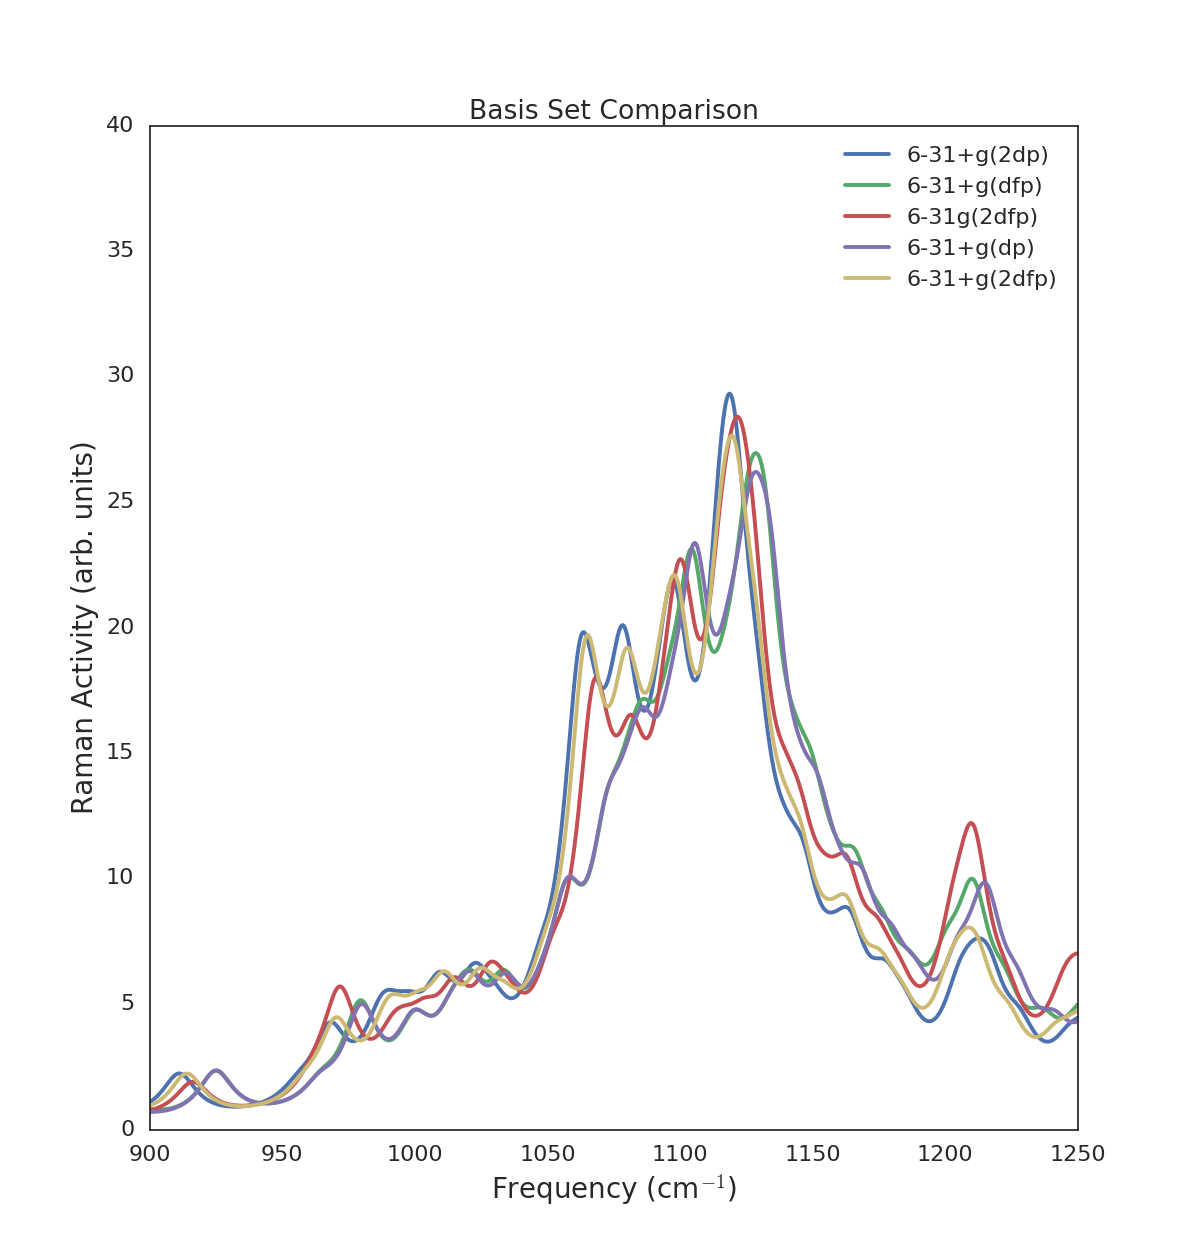
\includegraphics[width=0.7\linewidth]{basis_set_comparison}
\caption{Comparison of Raman spectra generated by different candidate basis sets.}
\label{fig:basis_set_comparison}
\end{figure}

\begin{table}[]
	\centering
	\caption{Times taken to calculate Raman spectrum with different basis sets for an identical cellobiose geometry at 280K.}
	\label{tbl:basis_sets}
	\begin{tabular}{@{}ll@{}}
		\toprule
		Basis Set      & Computation Time (hours) \\ \midrule
		6-31+G(2d,f,p) & 92                       \\
		6-31+G(d,f,p)  & 46                       \\
		6-31G(2d,f,p)  & 39                       \\
		6-31+G(2d,p)   & 31                       \\
		6-31+G(d,p)    & 13                       \\ \bottomrule
	\end{tabular}
\end{table}

The results of the comparison are shown in Figure \ref{fig:basis_set_comparison} and Table \ref{tbl:basis_sets}. These indicated that 6-31+G(2d,p) was the superior basis set for cellobiose simulation, delivering spectra nearly identical to those generated by 6-31+G(2d,f,p) while consuming 60\% less computer time. Therefore 6-31+G(2d,p) was used as the basis set for the bulk of the simulations.

\section{Vibrational Analysis}

Raman spectra were calculated directly from the simulation results by Gaussian. For this purpose, Gaussian employs a technique known as normal mode analysis (NMA). NMA depends on the fact that a molecule's vibrational modes are, mathematically speaking, normal to each other. In other words, they are independent, and each one has characteristics such as frequency that are independently calculable.

NMA assumes that the atoms in a molecule behave as a network of coupled three-dimensional harmonic oscillators, in which the movement of each atom (labeled with an index $i$) is affected by the position and movement of all the other atoms. To frame this mathematically, let each atom have instantaneous position coordinates $x_i, y_i, z_i$ centered about an equilibrium position denoted $x_{i,\mathrm{eq}}, y_{i,\mathrm{eq}}, z_{i,\mathrm{eq}}$. As harmonic oscillators, these atoms experience a force proportional to their displacements from their respective equilibrium positions, governed by a proportionality constant $k$. In addition, they vibrate with a characteristic frequency $\nu$ given by
\begin{equation}
\label{freq_eq}
4\pi \nu^2 mx = kx
\end{equation}
where $m$ is the atom's mass. If the atoms were considered to be simple and independent harmonic oscillators, as in the Einstein model of solids\cite{RefWorks:60}, $k$ would be simply a constant. However, in NMA, coupling dictates that $k$ is determined by the second derivative of the system's potential energy $V$ with respect to position. $V$ is a function of the overall configuration of the molecule; symbolically, $V = V(x_1, y_1, z_1 ... x_N, y_N, z_N)$. Therefore, to calculate all the force constants for all three directions of the $N$ atoms, we must take $3N$ derivatives of a function of $3N$ variables.

The result is a $3N \times 3N$ matrix of force constants describing the force each atom in the molecule feels, given an overall molecular configuration. This matrix is referred to as the Hessian, and it is of critical importance to a number of processes in computational chemistry, including energy minimization. If we denote the Hessian as $H$ and apply standard mass-weighting techniques, we can write the matrix representation of the molecular configuration as $X$ and use Equation \ref{freq_eq} to write
\begin{equation}
HX = 4\pi\nu X
\end{equation}
This is an eigenvalue equation. The eigenvalues of the Hessian are the neqative of the squared normal mode frequencies, and the eigenvectors are the mass-weighted normal coordinate displacements. In other words, solving this equation reveals how each normal mode vibrates, as well as the frequency at which it does so. With the eigenvalues and vectors in hand, Gaussian then proceeds to calculate how each vibrational mode affects the molecule's dipole moment and polarizability, producing IR and Raman intensities for each mode as well.

The reason this calculation must follow a wavefunction simulation phase is that the potential energy $V$ is determined by the wavefunction. The wavefunction determines the location and density of the electron cloud, which in turn determines how the atoms in the molecule interact. Therefore it is the combination of DFT and NMA that allows vibrational spectra to be accurately computed.

\section{Spectral Reconstruction}

It is important to note that normal mode analysis does not produce an actual visual spectrum. For each of an input molecule's vibrational modes, NMA generates a frequency, an IR intensity, a Raman activity level, and a set of vectors describing the vibration of itself in terms of atomic displacements. However, there is an accepted method for constructing a continuous spectrum based on this information. In essence, each vibrational mode is assumed to produce a peak (or trough, in the case of IR) in the spectrum with a Lorentzian profile, and the sum of these will reproduce an approximate spectrum \cite{RefWorks:55}.

A Lorentzian is a single-variable, three-parameter function similar to a Gaussian. It is described by the equation

\begin{equation}
L(x) = A\frac{\frac{1}{2}\Gamma}{(x-x_0)^2 + (\frac{1}{2}\Gamma)^2}
\end{equation}

\noindent where A is the amplitude, $\Gamma$ describes the width of the peak, and $x_0$ is the peak center. This function generates peaks with a distinctively pointed shape and long wings, illustrated in Figure \ref{fig:Lorentzian}. For a mode in the Raman spectrum, for example, peaks are recreated as Lorentzians centered at the mode frequency with an amplitude equal to the Raman activity. The only free parameter is the peak width; typically, this is chosen by investigators to best match the width of experimentally observed peaks. Typically this value is set between 8 to \SI{10}{cm^{-1}} \cite{RefWorks:33}.

A peak reconstruction proceeds in this fashion: let the vectors $F$ and $I$ represent the normal mode frequencies and their associated peak heights, and let $F_i$ and $I_i$ be the particular frequency and intensity for mode $i$. Assuming fixed peak width $\Gamma_0$, the peak $L_i$ is given as
\begin{equation}
L_i(x) = I_i\frac{\frac{1}{2}\Gamma_0}{(x-F_i)^2 + (\frac{1}{2}\Gamma_0)^2}
\end{equation}
Repeating this procedure for all $i$ (that is, all the vibrational modes), we can then derive a function $S$ that gives a continuous spectrum by summing:
\begin{equation}
S(x) = \sum_i I_i\frac{\frac{1}{2}\Gamma_0}{(x-F_i)^2 + (\frac{1}{2}\Gamma_0)^2}
\end{equation}
This function $S(x)$ represents the reconstructed spectrum. It takes a wavenumber in cm$^{-1}$ as input and returns the predicted intensity. In cases where frequencies are close together, the peak amplitudes will sum, and large super-peaks will form, as they do in real spectra.

This method has been proven effective for single sets of NMA output, but for the present work, we have hundreds of such outputs with which grapple. In the interest of isolating the effect of temperature on spectral features, we chose to handle this by averaging over the spectra computed at each temperature, yielding a set of second-order spectral functions that integrate all available information about spectral behavior at a given temperature.

Let $\Omega_T$ be the set of all computed spectral functions $S(x)$ at temperature $T$ and $\Omega_{T,i}$ be the $i$th element in the set. We can then construct the temperature's average spectrum $S_T(x)$ as:
\begin{equation}
S_T(x) = \frac{1}{|\Omega_T|}\sum_i \Omega_{T,t}(x)
\end{equation}
This procedure can be carried out for either Raman intensities or IR intensities. The resulting $S_T$ functions represent our model's prediction of the vibrational spectra of cellobiose at a temperature $T$.

In a similar fashion, the average vibrational displacement vectors can also be calculated. Let the total number of vibrational modes be $M$. At a temperature $T$, the $i$th vibrational mode of the $j$th simulation result contains a set of 3D eigenvectors $V_{j,i}$ numbered 1 through $N$, the number of atoms in the simulated molecule. The eigenvector with index $k$ describes the direction and magnitude of the motion $k$th atom during the mode's vibration. We wish to compute $\langle V_i \rangle_T$, the average set of atomic displacement vectors for mode $i$ at temperature $T$, taken over all the simulation results at $T$. Each entry in this set is given by the following formula:
\begin{equation}
\langle V_{i,k} \rangle_{T} = \frac{\sum_j^M V_{i,k}}{M}
\end{equation}
Calculating this quantity for each atom $k$ for each mode $i$, we can recompose the resulting vectors into a complete $\langle V \rangle_T$, which describes the average displacement vector for each vibrational mode at $T$.
\begin{figure}
\centering
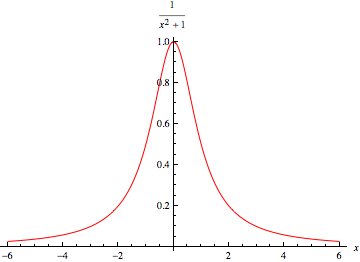
\includegraphics[width=0.7\linewidth]{Lorentzian}
\caption{Normalized Lorentzian function with center 0, width and amplitude 1.}
\label{fig:Lorentzian}
\end{figure}

\section{Summary}

To reiterate, the simulation protocol used for this work proceeds as follows: 

\begin{enumerate}
	\item Molecular dynamics is used to generate cellulose configurations at a given temperature.
	\item Cellobiose structures are extracted from the cellulose structure and capped with hydrogens.
	\item Density functional theory is used to calculate approximate wavefunctions for the cellobiose configurations.
	\item Normal mode analysis is used to compute Raman spectra from the simulated wavefunctions.
	\item Averaging techniques are used to compute representative spectra and vibrational modes for each simulated temperature.
\end{enumerate}

\section{Comparing to Experiment}

The spectral data produced by the protocol described above interesting in isolation, but even more so when compared to the equivalent experimental spectra. There are two complicating factors that must be addressed when carrying out such comparisons: slight deviations in predicted mode frequencies, and the arbitrary nature of Raman activity units. The first point refers to the widely observed fact that DFT/NMA calculations of mode frequencies tend to uniformly under or  overshoot experimentally observed frequencies by one to two percent. To aid comparison, the standard technique is to multiply each predicted frequency by a constant scaling factor, chosen to align some distinctive spectral feature. In this work, an empirically determined scaling factor of 1.017 was chosen to align the main low-frequency peak at approximately \SI{1100}{cm^{-1}}.

The second point refers to the fact that the absolute value of a peak's height in a Raman spectrum has no intrinsic meaning. Different calculational and experimental techniques will yield different numbers and use different units to report the Raman activity, but all of these are arbitrary. What matters from the standpoint of chemical insight is the relative height of each peak in the spectrum. To make this feature clear, we have adopted a simple spectral normalization procedure: we set the height of the tallest peak in the spectrum to be one, and take the lowest point in the spectrum to be zero. We then report the height at every other point as a unitless fraction of the maximum peak height. This way we can accurately compare any number of different spectral datasets, regardless of their native units or scales.

A final note is that certain experimental trials produce a spectra that sits on an elevated linear baseline, due to wide-spectrum polychromatic fluorescence (an effect not believed to be relevant to the pyrolysis process). No such baseline is produced in the simulation. Therefore, for these elevated trials a baseline-corrected spectrum is produced by subtracting the baseline value from each point in the spectrum.

The methods described above do have several limitations. Perhaps the most important is that, in this paradigm, the effects of inter-chain hydrogen bonding between strands of cellulose are ignored in the vibrational analysis stage. By sampling thermal configurations, we take into account the effects of hydrogen bonding on the starting molecular geometry, but certain vibrational modes that may be suppressed by that bonding are calculated to be active with this method, and vice versa. Also, the manual addition of carbon-linked hydrogens makes analysis of modes predominantly involving motion of these atoms unviable, as their positions do not necessarily reflect actual configurations seen at any real temperature. 
